\documentclass[review,12pt,number]{elsarticle}
% Elsevier submission format: review = double spacing + line numbers;
% number = numeric citations with elsarticle-num. For a double-column
% production-style preview use [3p,times,number] or [5p,times,number].
% Target journal: Knowledge-Based Systems (see cover_letter.md).
% Reference style note: this journal uses Elsevier numbered citations, matching
% elsarticle-num.bst below. No bst change is required for this target.
% Appendices A/B (statistics rationale, hyperparameters, full accuracy
% matrices) live in supplementary.tex, compiled separately.

\usepackage{amsmath,amssymb}
\usepackage{booktabs}
\usepackage{graphicx}
\usepackage{xcolor}
\usepackage{lineno}
\usepackage{url}
\graphicspath{{figs/}}

\newcommand{\todo}[1]{\textcolor{red}{[TODO: #1]}}
\newcommand{\delp}{DeLP}
\newcommand{\acc}{\mathrm{acc}}

\journal{Knowledge-Based Systems}

\begin{document}
\linenumbers

\begin{frontmatter}

\title{The Anchor Accumulation Problem:\\Bounded Anchor Sets, a Soft--Hard
Protection Law, and the Auditable Cost of Regularized Continual Learning}

\author[hnucm]{Ranxi Zhou}
\address[hnucm]{Hunan University of Chinese Medicine, 300 Xueshi Avenue,
Hanpu, Yuelu District, Changsha 410208, Hunan, China}
\cortext[cor1]{Corresponding author.}
\ead{zhouranxi@foxmail.com}

\begin{abstract}
Regularized continual-learning schemes that store one protection state
per task pay a cost that grows with sequence length. In usage-localized
elastic weight consolidation (\delp{}), per-neuron elastic anchors
persist at full weight as an elastic drag on later learning; a retention
decomposition $\bar a_T = \ell + \frac{T-1}{T}\,\mathrm{BWT}$ localizes
the cost in the \emph{learning term} $\ell$. We call this the
\emph{anchor accumulation problem} and study its repair: bounding the
anchor stack at $M$ entries. A FIFO budget recovers $+4.5$ and $+9.0$
points of final accuracy over unbounded \delp{} at $T{=}10$ and
$T{=}20$ ($M{=}5$; $n{=}10$ paired seeds; Wilcoxon $p{=}0.002$), and the
budget is a distinct knob from the elastic weight $\lambda$: it
controls the \emph{age structure} of forgetting, $\lambda$ its
\emph{amount}. Eviction design is ruled by one constraint: any criterion
keyed to current constraint mass grandfather-protects stale anchors and
evicts new ones at birth ($-34.5$ BWT), whereas age-first criteria are
immune. Sweeping online EWC's discount shows that discounting is itself
a \emph{soft} bound, and soft and hard bounds obey one log-linear law
between the learning term and the protected-mass horizon
($\ell \approx 84 - 11\ln h$, $R^2{=}0.99$): bounding accumulated anchor
mass, not eviction, is the active ingredient, and the explicit window
retains what a scalar discount cannot --- a discrete, named, policy-
selectable protection set readable from the stack trace. We report the
boundary honestly: on Split-CIFAR-100 under task-incremental evaluation,
a no-protection baseline stays above every protection arm, so the
budget result is internal to the protected family; the paper's
contribution is a \emph{knowledge-based diagnosis and audit framework}
--- when to protect, how to bound, which anchors survive --- not a
drop-in accuracy win.
\end{abstract}

\begin{keyword}
continual learning \sep elastic weight consolidation \sep
catastrophic forgetting \sep knowledge-based protection \sep
stability--plasticity dilemma
\end{keyword}

\end{frontmatter}

% ============================================================
\section{Introduction}
% ============================================================
\label{sec:intro}

Elastic weight consolidation (EWC)~\cite{kirkpatrick2017} and its
variants protect important parameters by penalizing departure from
values that served previous tasks. The idea originates in the
computational principles of synaptic memory consolidation~\cite{benna2016},
and a long line of work has since shaped it: synaptic
intelligence~\cite{zenke2017} accumulates path integrals online,
memory-aware synapses~\cite{aljundi2018} estimate sensitivity without
supervision, and context-dependent gating~\cite{masse2018} makes the
protection pathway itself task-conditional. Surveys
of the field~\cite{parisi2019,delange2022} document both the breadth of
these designs and how few of them are comparable under a common
protocol --- a gap our own audit of \delp{}~\cite{zhou2026delp} ran into
directly.

From a knowledge-based-systems perspective, the protection state that
these methods maintain \emph{is} a knowledge base: a growing, structured
store of what has been learned, consulted at every update, and
trusted in proportion to its age. Yet this knowledge base is rarely
treated as a first-class design object --- it is appended to, never
curated, bounded, or audited. This paper makes it the object of study.

\delp{}~\cite{zhou2026delp} localizes this protection to dendritic
compartments and weights each neuron's penalty by its measured usage
under previous tasks. The audit of the method
established that usage weighting survives a parameter-budget cap
($+1.79$, $p{=}0.005$ at twenty tasks) while the full dendritic chain
adds little once baselines share the hidden activation.

The same audit exposed a structural cost: \delp{} appends one anchor
set (posterior means and Fisher estimates) per task, so the elastic
drag on optimization grows with the sequence length $T$.
A decomposition of average retention,
%
\begin{equation}
\label{eq:decomp}
\bar a_T \;=\; \ell \;+\; \frac{T-1}{T}\,\mathrm{BWT},
\end{equation}
%
separates the \emph{learning term} $\ell$ (how well each task is
acquired at its boundary) from the backward-transfer term.
At ten tasks the losses of unbounded \delp{} are concentrated in $\ell$:
anchors from early tasks persist as elastic drag long after the tasks
they protect have been consolidated, and this is a property of the
protection scheme, not of the architecture.


This paper treats the anchor stack itself as the object of study.
We bound it at $M$ entries and ask four questions:
\textbf{(Q1)} Can the learning term be recovered by bounding, and at
what stability cost?
\textbf{(Q2)} Is the budget a redundant knob (a non-linear re-scaling
of $\lambda$), or does it control something $\lambda$ cannot?
\textbf{(Q3)} If the stack must be bounded, \emph{which} anchors should
be evicted?
\textbf{(Q4)} Does protection itself pay for its cost --- or does a
no-protection reference beat the entire protected family?

\paragraph{Contributions.}
Our contribution is a \emph{diagnosis-and-audit framework} for
protection state in regularized continual learning, together with a
quantitative account of when protection is worth its cost. We state the
boundary of the repair up front as a finding, not a footnote:
\begin{enumerate}
\item \textbf{A protection-must-justify-itself result.} On
Split-CIFAR-100 under task-incremental evaluation, a no-protection
baseline ($\lambda{=}0$) stays above every \delp{} arm including the
best budgeted one (Sec.~\ref{sec:exp-noprot}). The decomposition
explains why: at any $\lambda$, protection roughly halves the learning
term while retention in this regime is nearly free to forgo. We therefore
credit no protection benefit on that benchmark and recommend a
no-protection reference as a mandatory check for any regularized CL
pipeline --- a negative result we argue increases, rather than
decreases, the audit value of the framework.
\item \textbf{The anchor accumulation problem and its bounded repair.}
We identify the accumulation of full-weight per-task anchor stacks as
the binding constraint on the learning term of long sequences, and
introduce a family of eviction policies for anchor stacks. A FIFO
budget recovers $+4.5/+9.0$ points of final accuracy at $T{=}10/20$
over unbounded \delp{} ($n{=}10$ paired seeds; Wilcoxon $p{=}0.002$),
by recovering $+5.4/+15.2$ points of the learning term
(Eq.~\ref{eq:decomp}); the effect replicates on Fashion-MNIST
($+13.0$ at $M{=}2$) and, within the protected family, on
Split-CIFAR-100 (five of six bounded policies beat unbounded at
$T{=}20$, $M{=}2$, up to $+5.0$ points, Wilcoxon $p{=}0.002$).
\item \textbf{An eviction design space with one governing constraint.}
Through per-task accuracy profiles we show the budget controls the
\emph{age structure} of forgetting while $\lambda$ controls its total
amount (Fig.~\ref{fig:age}); and trace instrumentation
(Figs.~\ref{fig:stack},~\ref{fig:stackcifar}) shows that any criterion
keyed to an anchor's \emph{current constraint mass} fails
systematically: it grandfather-protects stale anchors and evicts new
ones at birth (BWT $-34.5$). Multiplicative age re-weighting does not
fix this; an age-first, mass-second criterion does. The primary key,
not the secondary signal, determines whether a criterion works.
\item \textbf{A soft--hard protection law.} Sweeping online EWC's
discount $\gamma$ shows a tuned discount overtakes the budget on
accuracy at matched forgetting --- and that discounting is itself a
\emph{soft} bound. Across soft (discount) and hard (window) bounds, the
learning term falls log-linearly in the protected-mass horizon
($\ell \approx 84 - 11\ln h$, $R^2{=}0.99$, per-seed $R^2 \geq 0.98$,
monotone at every grid $\lambda$; the same four-arm fit at $T{=}10$
gives a shallower slope, $-3.8$, $R^2{=}0.96$): bounding accumulated
anchor mass, not the mechanism enforcing it, is the active ingredient.
\item \textbf{Auditability as the residual value of explicit windows.}
Because the budget is a \emph{set} of named anchors rather than a
scalar discount, the protected mass is inspectable: which tasks are
still protected, which were evicted, and by which policy, are all
readable directly from the stack trace, and the forgetting profile the
trace predicts is the one measured ($8.6$ mean drop on the five
in-window tasks vs.\ $27.7$ on the five oldest evicted tasks). Fisher-cosine merging further decouples memory
from behavior: the penalty \emph{value} drops one-sidedly (up to
$64\%$, gradient unchanged) while accuracy stays indistinguishable from
unbounded. What the explicit window retains over a tuned discount is
thus exactly the knowledge representation: a discrete, named,
policy-selectable protection set.
\end{enumerate}

% ============================================================
\section{Related work}
% ============================================================
\label{sec:related}

\begin{sloppypar}
\paragraph{Regularization-based continual learning.}
EWC~\cite{kirkpatrick2017} places a quadratic penalty around posterior
estimates of previous tasks; SI~\cite{zenke2017} accumulates
path-integral importances online; MAS~\cite{aljundi2018} estimates
sensitivity unsupervised. Anchor accumulation is not specific to
\delp{}: any scheme that stores per-task quadratics pays storage
$O(T)$ and, if all terms persist at full weight, an increasingly
rigid objective. Online EWC~\cite{chaudhry2018} addresses the storage
axis by collapsing the stack into a single running posterior; with a
discount $\gamma{<}1$ its Fisher mass is geometrically bounded, which
makes it a \emph{soft} bound on the same accumulated mass we diagnose
(Sec.~\ref{sec:exp-references}). Bounded anchor sets are complementary:
they keep per-task terms and bound their number.

\paragraph{Recent continual-learning methods.}
Recent work treats the
stability--plasticity trade-off from several angles, and our work is
complementary to all of it because it targets the \emph{accumulation
mechanism} of a regularizer rather than the network parameterisation.
Forget to Learn~\cite{hassan2025f2l} circumvents the conflict in
continuous unsupervised domain adaptation by active forgetting plus
conflict-free distillation; {TIPS}~\cite{feng2026tips} selects prompts at
two granularities to rebalance stability and plasticity in prompt-based
continual learning; a dual-learner with cumulative parameter
averaging~\cite{sun2026dlcpa} pairs a plastic learner with a stable one;
and {LoRAC}~\cite{ling2026lorac} constrains critical parameter changes
under orthogonal {LoRA} tuning. These are all \emph{architectural or
replay-side} remedies. Ours is complementary: we ask what happens
\emph{inside} a regularizer that accumulates one anchor set per task,
and we show that the accumulation itself --- not the eviction rule,
not the discount schedule --- is what costs plasticity. We cite the
rehearsal-side family~\cite{buzzega2020der} as the reference point that
makes exemplar-free regularizer comparisons legible: a strong baseline
of this kind forces one to state honestly in which regime a comparison
holds.
\end{sloppypar}
\paragraph{Parameter isolation and budgeting.}
PackNet~\cite{mallya2018} and HAT~\cite{serra2018} budget capacity
explicitly. Our contribution differs: the budgeted object is the
\emph{protection} state, not the network capacity, and eviction can
be nearly free when the penalty is combined correctly (merge).

\paragraph{Dendritic computation.}
The dendritic substrate is not decorative. Pyramidal neurons are
multicompartmental systems in which local dendritic potentials shape
integration at the soma~\cite{chang1951,poirazi2003,beniaguev2021}, and
these computations are measurable \emph{in vivo}
rather than merely modeled: dendritic activity in the cortex is
multiplexed and globally modulated~\cite{ujfalussy2018}, and it
computes abstract rules~\cite{zhang2026}. Reviews of dendritic
computation~\cite{london2005,poirazi2020} and of its engineering
exploitation~\cite{cardwell2025,boyle2025,baek2024,boahen2022} make the
relevant point for us: the compartment is a computational unit with its
own timescales, so protecting it with a task-wise snapshot is a
substantive modeling choice rather than an implementation detail.
Active-dendrite networks~\cite{iyer2022,onasch2026} provide the
architectural substrate; \delp{}'s audit~\cite{zhou2026delp}
established which part of the dendritic chain carries the benefit.

\paragraph{Scope of this manuscript in relation to the author's precursor
work.} Two earlier Zenodo preprints by the same author
\cite{zhou2026delp,zhou2026seg} audited, respectively, which component of the
dendritic chain carries the DeLP benefit and how that benefit distributes across
input segments. Both are diagnostic studies of \emph{where} the benefit
originates; neither examines what happens to a stack of anchors as the task
sequence grows. The present manuscript takes the opposite direction. Its
subject is the cost that \emph{any} stack-building scheme pays over a long
sequence --- the anchor accumulation problem --- and its object is the repair
for that cost: bounding the anchor stack at $M$ entries, the eviction criteria
that decide which anchors survive, and the resulting law relating soft and
hard protection bounds. All experiments, analyses, figures, and text in the
present manuscript are new; the precursor audits are cited as prior work and
are not extended, reproduced, or reused here.

% ============================================================
\section{Background: \delp{} and anchor accumulation}
% ============================================================
\label{sec:background}

\paragraph{Setup.}
A network is trained on a sequence of $T$ tasks (permuted MNIST /
Fashion-MNIST). \delp{} freezes dendritic segments unused by the
current task and adds, after each task $t$, an anchor set
$\mathcal{A}_t = \{(\theta_t, F_t)\}$ (parameter snapshot and Fisher
diagonal). The protection objective during task $t$ is
%
\begin{equation}
\label{eq:delp}
\mathcal{L}_t(\theta) \;=\; \mathcal{L}_t^{\text{task}}(\theta)
\;+\; \frac{\lambda}{2}\sum_{k<t}\sum_i F^{(k)}_i
      \,(\theta_i - \theta^{(k)}_i)^2 ,
\end{equation}
%
where the inner sum runs over the accumulated stack
$\mathcal{A}_1, \dots, \mathcal{A}_{t-1}$: the penalty is
\emph{unbounded} in $T$, both in storage and in constraint mass.

\paragraph{Where the cost lands.}
Following~\cite{zhou2026delp}, average retention decomposes as
Eq.~\ref{eq:decomp}. % cite numbers: at T=10 unbounded DeLP:
% acc 55.3, BWT -5.5, ell 60.2; at T=20: 33.7 / -4.4 / 37.9
At fixed $\lambda{=}5000$ the learning term of unbounded \delp{}
falls from $59.2$ at $T{=}10$ to $37.7$ at $T{=}20$ --- a
$21.5$-point drop that compounds with sequence length, exactly the
signature of drag that accumulates with every finished task;
anchored identity Eq.~\ref{eq:decomp} attributes the gap to $\ell$,
not BWT. We call this the \emph{anchor accumulation problem}.

% ============================================================
\section{Bounded anchor sets}
% ============================================================
\label{sec:method}

\paragraph{Budgeted stacks.}
We replace the unbounded stack with a bounded one of size $M$.
After appending the anchor for task $t$, if $|\mathcal{A}| > M$ an
\emph{eviction policy} removes or combines entries:
%
\begin{equation}
\label{eq:budget}
\mathcal{A} \leftarrow \mathsf{evict}_\pi\!\left(
\mathcal{A} \cup \{(\theta_t, F_t)\},\, M \right).
\end{equation}

\paragraph{Policies.}
Table~\ref{tab:policies} defines the six policies we compare. They
span the design space along one axis: \emph{what signal drives the
choice} --- age (fifo), chance (random), current constraint mass
(redun), pairwise redundancy (merge), or combinations of age and
mass (agew, agew2).

\begin{table}[t]
\centering\small
\caption{Eviction policies for a stack over budget. Constraint mass
$m_k = \sum_i F^{(k)}_i (\theta^{\text{now}}_i-\theta^{(k)}_i)^2$ is
measured at eviction time.}
\label{tab:policies}
\begin{tabular}{llp{8.2cm}}
\toprule
Policy & Key & Rule (when $|\mathcal{A}|>M$) \\
\midrule
unbounded & --- & never evict (original \delp{}) \\
fifo      & age & evict the oldest anchor \\
random    & --- & evict uniformly at random \\
redun     & mass & evict $\arg\min_k m_k$ \\
agew      & mass $\times$ age & evict $\arg\min_k m_k \cdot (k{+}1)$,
    oldest $k{=}0$ \\
agew2     & age $\to$ mass & evict oldest anchor with below-median $m_k$;
    fallback fifo \\
merge     & redundancy & merge the pair with most similar $F$
    (cosine): $F \leftarrow F_i + F_j$, $\theta \leftarrow$ weighted
    mean; repeat \\
\bottomrule
\end{tabular}
\end{table}

\begin{sloppypar}
\paragraph{Instrumentation.}
Each anchor carries an \emph{origin} tag (the task that created it),
and we record the surviving-origin set after every phase
(\texttt{survivor\_history}). This turns the eviction dynamics into a
directly observable object (Fig.~\ref{fig:stack}).
\end{sloppypar}

% ============================================================
\section{Experiments}
% ============================================================
\label{sec:exp}

\paragraph{Protocol.}
Permuted-MNIST and Fashion-MNIST, $T \in \{10, 20\}$; architecture,
optimizer, permutation generation, and evaluation identical to the
\delp{} audit protocol~\cite{zhou2026delp}; $\lambda{=}5000$ unless stated. Every arm runs at the pipeline's
\emph{default} hidden-layer gain --- the uncalibrated condition of the
audit's calibration protocol~\cite{zhou2026delp} --- and no arm is
gain-tuned within this study; since the gain is shared, the confound
the audit documented (a single gain scalar moves accuracy by more than
the entire method) cannot differentially favor any arm, only shift all
arms together. Paired comparisons use identical seeds.
Budgets $M \in \{2, 5\}$ anchor the main grid; a seven-point
dose--response sweep $M \in \{2,3,4,5,6,8,10\}$ ($T{=}20$,
$\lambda{=}5000$; Sec.~\ref{sec:exp-knobs}) fills the interior, and no
$M$ was tuned post hoc.
Section~\ref{sec:exp-cifar} states the Split-CIFAR-100 protocol
separately (different backbone and protection pathway).

\subsection{Bounding recovers plasticity (Q1)}
\label{sec:exp-main}

\begin{table}[t]
\centering\small
\caption{Paired fifo--unbounded deltas, $M{=}5$, $\lambda{=}5000$,
$n{=}10$ seeds. $t(9)$ is the paired t statistic; $W_p$ is the
two-sided p-value of the Wilcoxon signed-rank test on the same paired
deltas, and $W_p^{\mathrm{SW}}$ is the Shapiro--Wilk p-value on those
deltas (normality of the paired difference, on which the t test
depends).}
\label{tab:paired}
\begin{tabular}{lccccc}
\toprule
Arm & $\Delta\acc$ & $t(9)$ & $W_p$ & $W_p^{\mathrm{SW}}$ & $\Delta$BWT \\
\midrule
fifo $T{=}10$ & $+4.51\pm0.67$ & $21.4$ & $0.002$ & $0.024$ & $-1.50\pm0.49$ \\
fifo $T{=}20$ & $+8.98\pm1.49$ & $19.1$ & $0.002$ & $0.992$ & $-7.20\pm1.97$ \\
\bottomrule
\end{tabular}
\end{table}

\begin{table}[t]
\centering\small
\caption{Policy grid, $M{=}5$, $\lambda{=}5000$, mean $\pm$ sd over
$n{=}3$ seeds. $\ell$ = learning term (mean accuracy at task
boundaries). agew is bit-identical to redun, as predicted in
Sec.~\ref{sec:exp-criteria}.}
\label{tab:grid}
\begin{tabular}{llccc}
\toprule
$T$ & Arm & BWT & $\acc$ & $\ell$ \\
\midrule
10 & unbounded & $-5.5\pm0.6$   & $55.3$ & $60.2$ \\
10 & fifo      & $-6.6\pm0.9$   & $59.7$ & $65.6$ \\
10 & random    & $-9.1\pm2.6$   & $60.2$ & $68.4$ \\
10 & redun     & $-18.3\pm0.8$  & $53.6$ & $70.1$ \\
10 & agew      & $-18.3\pm0.8$  & $53.6$ & $70.1$ \\
10 & agew2     & $-8.4\pm0.9$   & $60.8$ & $68.3$ \\
10 & merge     & $-5.5\pm0.6$   & $55.3$ & $60.3$ \\
\midrule
20 & unbounded & $-4.4\pm1.0$   & $33.7$ & $37.9$ \\
20 & fifo      & $-10.2\pm1.9$  & $43.4$ & $53.1$ \\
20 & random    & $-13.5\pm0.4$  & $42.0$ & $54.8$ \\
20 & redun     & $-30.2\pm0.4$  & $36.3$ & $65.0$ \\
20 & agew      & $-30.2\pm0.4$  & $36.3$ & $65.0$ \\
20 & agew2     & $-16.5\pm0.3$  & $42.3$ & $58.0$ \\
20 & merge     & $-4.5\pm0.9$   & $33.6$ & $37.9$ \\
\bottomrule
\end{tabular}
\end{table}

Table~\ref{tab:paired}: a FIFO budget at $M{=}5$ trades $1.5/7.2$ points
of BWT for $+4.5/+9.0$ accuracy. The mechanism is the learning term:
$\ell$ rises by $+5.4$ and $+15.2$, exactly the recovery predicted if
accumulated elastic drag were the binding constraint
(Sec.~\ref{sec:background}); the grid in Table~\ref{tab:grid} shows the
same signature for every bounded arm.
Eq.~\ref{eq:decomp} is an accounting identity, so the decomposition
alone is not evidence; the causal claim rests on the eviction traces
(Sec.~\ref{sec:exp-criteria}) and on the $\lambda$-by-budget
interaction (Sec.~\ref{sec:exp-knobs}), which localize \emph{when}
the learning term moves --- namely when anchors are actually retired.
Corrected SI at $T{=}10$ ($\lambda{=}100$) reaches $40.3\%$.

\subsection{Single-anchor schemes: the stack vs.\ its alternatives}
\label{sec:exp-references}

Because the diagnosis targets the \emph{stack}, we also ran two
protection schemes that cannot accumulate one. Both use the identical
architecture, protocol, and $\lambda$ grid ($n{=}10$ paired seeds):
plain EWC, which keeps only the most recent task's Fisher and anchor
(no accumulation, no running Fisher update --- distinct from the
original accumulated variant of~\cite{kirkpatrick2017}), and online
EWC \cite{chaudhry2018} with $\gamma \in \{0.5, 0.9, 1\}$, which
collapses the stack into a single running posterior with geometrically
discounted Fisher accumulation. All arms share the identical
$\lambda$ grid and are compared at each scheme's best grid value, so
no scheme is disadvantaged by another's tuning.

Plain EWC posts the highest final accuracy
of any arm ($68.3$--$71.1$ at $T{=}10$, $56.4$--$59.4$ at $T{=}20$,
best at $\lambda{=}1000$) by maximizing $\ell$ ($81$--$85$): with no
stack there is no accumulation --- and no retention either, at
$3$--$5\times$ the forgetting of unbounded \delp{} (BWT
$-15.8/-25.7$ at its best $\lambda$ vs.\ $-5.5/-4.4$). Under the
final-accuracy metric the learning-term dominance outweighs retention;
a reader who weights BWT equally would rank it last.

Online EWC at its best grid value ($\lambda{=}1000$) reaches $67.5/46.0$:
at $T{=}10$ it is statistically indistinguishable from \delp{}-fifo at
the same $\lambda$ ($67.4$; paired $t(9){=}-0.3$); at $T{=}20$ fifo is
$+3.5$ ahead ($t(9){=}7.0$). A collapsed posterior thus recovers most of
the plasticity, but it posts neither the best long-sequence accuracy
nor, by construction, any anchor accumulation problem to cure. Its
forgetting is not unstructured: per-task forgetting (peak minus final
accuracy; $T{=}20$, $\lambda{=}1000$, $n{=}10$) concentrates on older
tasks for every arm, with drop--age correlations of $-0.94$ (plain),
$-0.79$ (\delp{}-fifo), $-0.70$ (online EWC), and $-0.43$ (unbounded).

\subsection{The soft--hard protection law}
\label{sec:exp-law}

Sweeping the discount shows that the collapsed posterior does have an
age knob after all: lowering $\gamma$ to $0.9$ and $0.5$
raises $\ell$ from $51.1$ to $56.6$ and $76.1$ ($T{=}20$,
$\lambda{=}1000$), and at $\gamma{=}0.5$ online EWC overtakes
\delp{}-fifo at every grid cell we tested (paired $+4.7$ to $+7.9$,
all $|t(9)|\geq10.4$) at essentially matched BWT ($-19.5$ vs.\
$-19.7$). Discounting, however, is itself a bound: with geometrically
decayed Fishers the accumulated mass converges to an effective horizon
of ${\approx}\,1/(1-\gamma)$ tasks, so $\gamma{<}1$ is a \emph{soft}
counterpart of the eviction window.

The two mechanisms turn out to be interchangeable points on one curve.
Across all five bounded-mass
arms at $\lambda{=}1000$, $\ell$ is log-linear in the protected
horizon $h$ ($h{=}1$ plain, $h{=}2$ for $\gamma{=}0.5$, $h{=}5$ for
the window, $h{=}10$ for $\gamma{=}0.9$, $h{=}20$ unbounded):
\begin{equation}
\label{eq:law}
\ell \;\approx\; 84 - 11\ln h, \qquad R^2 = 0.99,
\end{equation}
a fit that holds for
every seed individually (per-seed $R^2 \geq 0.98$, slope
$-10.9\pm0.6$); the same four-arm fit at $T{=}10$ (excluding
$\gamma{=}0.9$, whose $\ell$ sits $0.7$ below the line) gives a
shallower slope ($-3.7$, $R^2{=}0.95$), consistent with a 10-task
sequence probing a shorter stretch of the horizon; and the ordering is
monotone at every grid $\lambda$ (mean-fit $R^2$
$0.99/0.94/0.80$ as $\lambda$ tightens). Bounding accumulated anchor
mass --- not
the mechanism that enforces the bound --- is the active ingredient,
and the soft bound is the stronger remedy on final accuracy in this
regime.

What the explicit window retains is auditability and
policy-level choice: its protection set is discrete and named by the
survivor trace; the forgetting profile it produces is the one the
trace predicts ($8.6$ mean drop on the five in-window tasks vs.\ $27.7$
on the five oldest evicted tasks; $T{=}20$, $\lambda{=}1000$); and the
eviction key can be swapped (age, mass) or the stack
merged without touching the update rule. The object studied here
remains the stack; the budget is one of two cures, and on this
benchmark the simpler one wins.

\subsection{Budget vs.\ $\lambda$: two orthogonal knobs (Q2)}
\label{sec:exp-knobs}

Fig.~\ref{fig:pareto} shows the Pareto plane; Fig.~\ref{fig:age} the
per-task accuracy profiles; Table~\ref{tab:lambda} the $\lambda$
interaction.

\paragraph{Dose--response.}
A seven-point sweep at $T{=}20$, $\lambda{=}5000$ ($n{=}10$) shows the
budget's effect is monotone across the whole interior, not an artifact
of two extreme points: final accuracy $52.1, 48.9, 45.0, 42.4, 40.2,
36.5, 35.1$ for $M{=}2,3,4,5,6,8,10$, with BWT recovering
$-25.0 \to -5.2$ as the window widens toward $M{=}10$; every $M$
remains significantly above unbounded at the same
$\lambda{=}5000$ ($33.4$; paired $t\geq 9.1$ at every $M$,
from $t{=}55.4$ at $M{=}3$ down to $t{=}9.1$ at $M{=}10$, approaching
the window's own limit).

\begin{figure}[t]
\centering
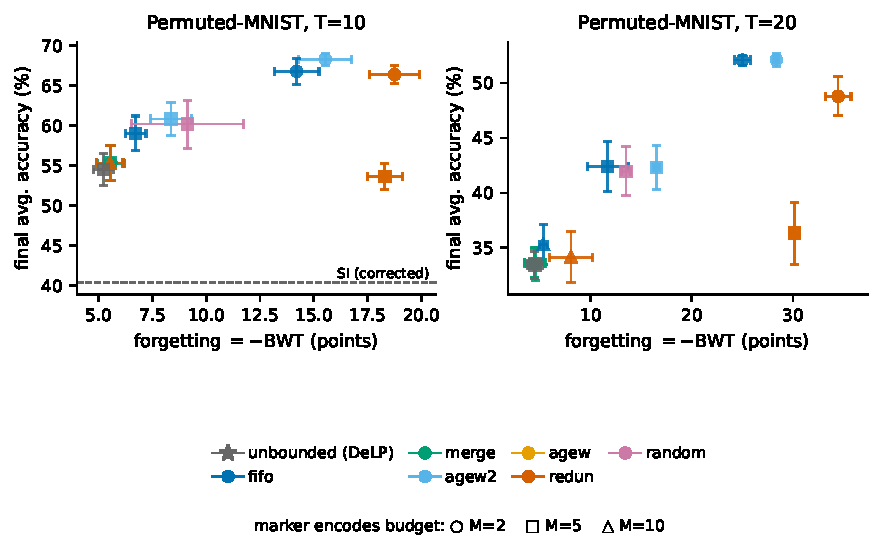
\includegraphics[width=\linewidth]{fig1_pareto.pdf}
\caption{Accuracy--forgetting trade-off on Permuted-MNIST. Color
encodes policy; marker encodes budget $M$. Error bars: sd over seeds
($n{=}10$ for unbounded/fifo $M{=}5$; else $n{=}3$). The smaller
budget $M{=}2$ trades BWT for accuracy at both budgets in the same
direction; merge coincides with
unbounded at every $M$; redun sits dominated.}
\label{fig:pareto}
\end{figure}

\begin{table}[t]
\centering\small
\caption{$\lambda$ interaction ($M{=}5$, $n{=}10$ paired seeds): the
fifo advantage is positive at every $\lambda$ and grows with $T$
(all paired $t(9)\geq 11$, $p<10^{-6}$).}
\label{tab:lambda}
\begin{tabular}{llccc}
\toprule
$\lambda$ & $T$ & unbounded BWT/$\acc$ & fifo BWT/$\acc$ & $\Delta\acc$ \\
\midrule
1000  & 10 & $-11.6 / 63.9$ & $-10.8 / 67.4$ & $+3.5$ \\
5000  & 10 & $-5.2 / 54.5$  & $-6.7 / 59.0$  & $+4.5$ \\
20000 & 10 & $-1.9 / 49.0$  & $-4.0 / 53.1$  & $+4.1$ \\
1000  & 20 & $-13.8 / 38.6$ & $-19.7 / 49.5$ & $+10.9$ \\
5000  & 20 & $-4.5 / 33.4$  & $-11.7 / 42.4$ & $+9.0$ \\
20000 & 20 & $-1.5 / 29.8$  & $-6.6 / 37.3$  & $+7.5$ \\
\bottomrule
\end{tabular}
\end{table}

The fifo advantage is robust to the choice of $\lambda$: even granting
unbounded \delp{} its best grid value at each $T$ ($\lambda{=}1000$, the
value at which unbounded is strongest at $T{=}20$), fifo retains a
$+10.9$-point advantage there (and $+3.5$ at $T{=}10$). That the
unbounded-optimal $\lambda$ must drift downward as $T$ grows is itself
a symptom of accumulating rigidity: the protection budget has to be
relaxed sequence-wide to compensate for anchors that a bounded scheme
would simply retire.

Both knobs move the system along a protection--plasticity spectrum,
but they are not re-parameterizations of one another. At matched
plasticity recovery, the two knobs produce \emph{different age
structures} of forgetting (Fig.~\ref{fig:age}):
$\lambda{=}1000$ scales down protection uniformly --- the profile
keeps its steep age gradient ($41.8$-point spread, oldest tasks at
66--83\%, newest at 41--50\%) --- while fifo $M{=}2$
redistributes forgetting onto the oldest tasks, flattening the
profile ($22.1$-point spread).
No value of $\lambda$ produces the flat profile, and no value of $M$
produces the uniform scaling.

\begin{figure}[t]
\centering
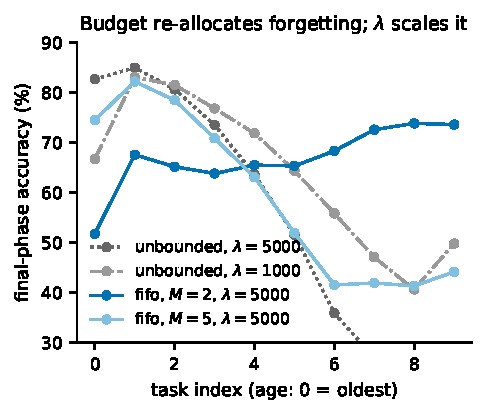
\includegraphics[width=0.62\linewidth]{fig2_ageprofile.pdf}
\caption{Final-phase accuracy per task ($T{=}10$, $n{=}10$).
$\lambda$ knobs (gray) translate the profile; budget knobs (blue)
flatten it: forgetting is re-allocated to the oldest tasks.}
\label{fig:age}
\end{figure}

\subsection{Which anchors to evict (Q3)}
\label{sec:exp-criteria}

\begin{figure*}[t]
\centering
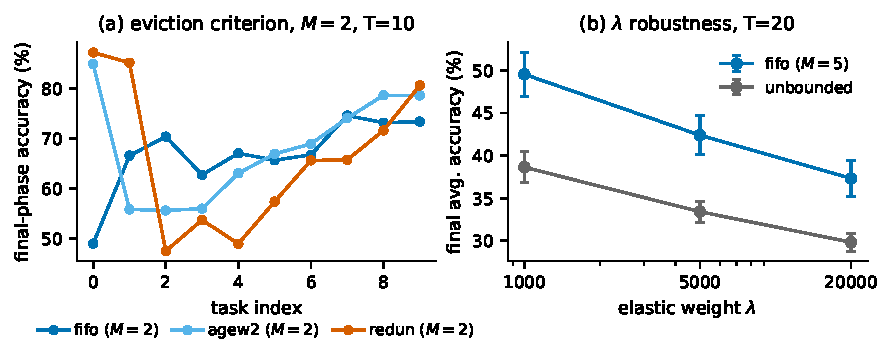
\includegraphics[width=\linewidth]{fig3_criteria.pdf}
\caption{(a) Mass-keyed eviction (redun) grandfather-protects the
first $M$ tasks and erases the middle; age-first criteria (fifo,
agew2) spread the cost. (b) The fifo advantage over unbounded holds
at every $\lambda$.}
\label{fig:criteria}
\end{figure*}

\paragraph{The grandfathering trap.}
Mass-keyed eviction is not a straw man: ``drop the anchor that
constrains least'' is the natural heuristic, homologous to
low-sensitivity-first intuitions in pruning and in MAS-style
importance estimates, and it is what a practitioner would try first.
Its systematic failure is the point. Constraint mass $m_k$
(Table~\ref{tab:policies}) is measured at
eviction time and is a function of staleness: anchors created before
the budget first binds have $\theta^{(k)}$ far from
$\theta^{\text{now}}$ and permanently large $m_k$; anchors created
\emph{after} the stack is full have $\theta^{(k)} \approx
\theta^{\text{now}}$ and $m_k \approx 0$. Mass-keyed eviction
therefore preserves exactly the stalest anchors and evicts new ones
\emph{at birth}: redun's stack freezes at
$\{\mathcal{A}_1, \mathcal{A}_2\}$ (Fig.~\ref{fig:stack}), the first
two tasks keep strong protection (87/85\% final accuracy at
$M{=}2$), and tasks created later lose all protection within one
phase (final accuracy 19--25\%), driving BWT to $-34.5$ at $T{=}20$
despite the \emph{highest} $\ell$ of any arm.

\paragraph{Re-weighting mass by age does not help.}
agew (mass $\times$ age-rank) is \emph{bit-identical} to redun across
all seeds and configurations: mass differences span orders of
magnitude and swamp the age factor, so the argmin never flips.
Any criterion with mass as the primary key inherits the trap.

\paragraph{Age-first criteria close the matrix.}
agew2 (oldest anchor with below-median mass; fallback fifo) behaves
like fifo ($\pm 1.5$ points): at $M{=}2$ its stack is
$\{\mathcal{A}_1, \mathcal{A}_T\}$ --- the oldest anchor's mass is
always above median and survives, everything in between dies at
birth. Table~\ref{tab:criteria} summarizes the resulting
$2{\times}2$: the primary key, not the secondary signal, determines
whether a criterion works.

\begin{table}[t]
\centering\small
\caption{Criteria $2{\times}2$: primary key (rows) $\times$ secondary
signal (columns). Only age-first criteria avoid the trap.
$T{=}10$/$T{=}20$ BWT and accuracy, $M{=}2$ or $M{=}5$ as marked,
$n{=}3$.}
\label{tab:criteria}
\begin{tabular}{lll}
\toprule
Primary key & Secondary & Outcome \\
\midrule
mass  & ---   & redun: grandfathering, BWT $-30.2$ ($M5$, T20) \\
mass  & $\times$ age & agew $\equiv$ redun (bit-identical) \\
age   & ---   & fifo: sliding window, BWT $-10.2$ ($M5$, T20) \\
age   & median mass & agew2 $\approx$ fifo ($\pm1.5$ pts) \\
\bottomrule
\end{tabular}
\end{table}

\begin{figure*}[t]
\centering
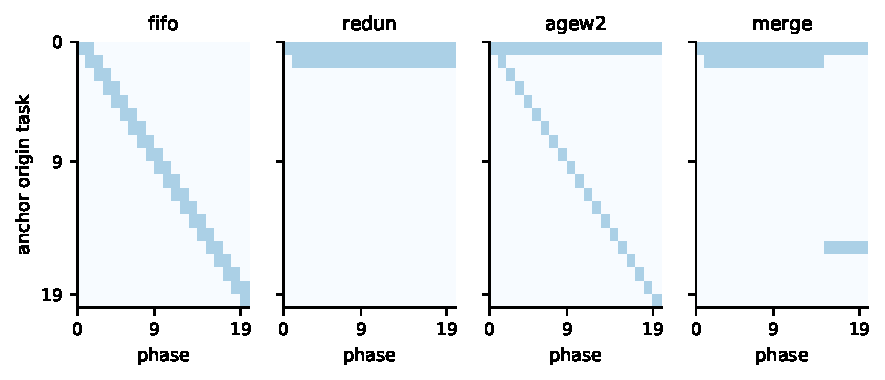
\includegraphics[width=\linewidth]{fig4_stacktrace.pdf}
\caption{Anchor-stack composition over the task sequence ($T{=}20$,
$M{=}2$, seed 0; identical for other seeds). Each column lists which
anchors (by creation task) are alive at the end of each phase. fifo
is a pure sliding window; redun freezes on the first two anchors
(evicting every later anchor at birth); agew2 protects the oldest and
the newest; merge partially grandfather-protects.}
\label{fig:stack}
\end{figure*}

\subsection{Memory without behavior change: merge}
\label{sec:exp-merge}

Merging the most Fisher-similar pair removes exactly the cross term
between the merged anchors. Penalty instrumentation over $40$ runs
($T \in \{10,20\}$, $M \in \{2,5\}$, $n{=}10$; exactly $T{-}M$ merges
per run) makes the change quantitative: the penalty's \emph{value} drops
one-sidedly --- never increases --- with per-run maximum relative
drops of $43$--$45\%$ at $M{=}2$ (worst case $64\%$) and $18$--$34\%$
at $M{=}5$, and $77\%$ of individual merges change that value. The
change is \emph{value-level only}: merging preserves the first-order
quadratic regularizer (the gradient $\nabla_\theta$ of the penalty is
unchanged), shifting only the parameter-independent constant, which
has zero effect on SGD. The removed mass is precisely the redundancy
the merge detected; the
accuracy trajectory nonetheless remains indistinguishable from
unbounded at every $M$ (Table~\ref{tab:grid}) while storing
$M \ll T$ anchors ($-75\%$ at $T{=}20$, $M{=}5$).
Merge and fifo are complementary: merge buys storage at a measured,
behaviorally invisible penalty reduction but recovers no plasticity;
fifo buys plasticity at a BWT price but no storage reduction.

\subsection{Generality check: Fashion-MNIST}
\label{sec:exp-fashion}

Fashion-MNIST, $T{=}10$, $n{=}7$ paired seeds (3--9): unbounded
$35.6\pm1.1$; fifo $M{=}5$ $38.4\pm1.6$ ($+2.8$, $t(6){=}10.5$); fifo
$M{=}2$ $48.6\pm2.1$ ($+13.0$, $t(6){=}16.2$). The budget
effect replicates and amplifies as the budget shrinks.

\subsection{Generalization to Split-CIFAR-100}
\label{sec:exp-cifar}

\paragraph{Protocol.}
Split-CIFAR-100, $T \in \{10, 20\}$: the 100 classes are split into
$T$ contiguous slices of $100/T$ classes each ($10$ classes/task at
$T{=}10$, $5$ classes/task at $T{=}20$; the code partitions a
random permutation of the 100 classes into $T$ blocks), ResNet-18
adapted to $32{\times}32$ inputs with GroupNorm in place of BatchNorm
--- running statistics are buffers that drift under later tasks and
silently destroy protected tasks while the anchored weights themselves
are held fixed, so they are excluded by design. Evaluation and training
are task-incremental with a masked softmax head: each task computes its
loss only over its own $100/T$ classes, so head rows of past tasks receive
no gradient and are protected by construction; anchors therefore cover
the backbone only, and forgetting can propagate exclusively through
the shared trunk --- exactly the pathway the anchor stack governs.
Fisher diagonals are rescaled to unit global mean (one scalar over all
parameters), making $\lambda$ backbone-independent; gradients are
clipped at norm 5. SGD, five epochs per task, $\lambda{=}0.1$ (chosen
by an independent calibration sweep on unbounded \delp{} only),
$n{=}10$ seeds; eviction policies, origin instrumentation, and paired
evaluation identical to the MNIST experiments. Unbounded \delp{} never
evicts, so its $M$ is inert (final stack size $T$ in every run); it is
materialized once per $T$ and serves as the reference for both
budgets. All CIFAR comparisons are task-incremental (masked head);
absolute accuracies are therefore not comparable to the
class-incremental Split-CIFAR-100 literature, and every claim in this
section is a within-family, same-protocol paired comparison.

\begin{table}[t]
\centering\small
\caption{Split-CIFAR-100, $\lambda{=}0.1$: final accuracy, mean
$\pm$ sd over $n{=}10$ seeds; parenthesized values are the paired
difference $\Delta\acc$ against unbounded \delp{} at the same seed
(quoted in text with the paired $t(9)$ and the two-sided Wilcoxon
signed-rank $p$-value).}
\label{tab:cifar}
\setlength{\tabcolsep}{4pt}
\footnotesize
\begin{tabular}{lcccc}
\toprule
& \multicolumn{2}{c}{$T{=}10$} & \multicolumn{2}{c}{$T{=}20$} \\
\cmidrule(r){2-3}\cmidrule(l){4-5}
Policy & $M{=}2$ & $M{=}5$ & $M{=}2$ & $M{=}5$ \\
\midrule
unbounded & \multicolumn{2}{c}{$23.3\pm2.6$} & \multicolumn{2}{c}{$29.8\pm4.2$} \\
fifo   & $24.8\pm2.8$ ($+1.5$) & $23.5\pm2.6$ ($+0.2$) &
         $\mathbf{34.8\pm4.8}$ ($+5.0$) & $32.2\pm4.3$ ($+2.4$) \\
random & $24.7\pm2.4$ ($+1.5$) & $22.4\pm2.7$ ($-0.9$) &
         $33.4\pm3.9$ ($+3.6$) & $32.2\pm4.7$ ($+2.4$) \\
redun  & $24.0\pm2.5$ ($+0.7$) & $23.6\pm2.0$ ($+0.3$) &
         $33.2\pm4.7$ ($+3.4$) & $32.9\pm3.3$ ($+3.1$) \\
merge  & $22.3\pm1.7$ ($-1.0$) & $21.8\pm3.2$ ($-1.5$) &
         $30.8\pm5.2$ ($+1.0$) & $29.3\pm3.4$ ($-0.5$) \\
agew   & $24.0\pm3.8$ ($+0.7$) & $22.7\pm3.4$ ($-0.6$) &
         $34.0\pm4.3$ ($+4.2$) & $31.6\pm3.7$ ($+1.8$) \\
agew2  & $23.7\pm2.6$ ($+0.4$) & $22.3\pm3.3$ ($-1.0$) &
         $32.5\pm3.7$ ($+2.7$) & $31.1\pm3.4$ ($+1.3$) \\
\bottomrule
\end{tabular}
\end{table}

\begin{sloppypar}
\paragraph{The budget effect strengthens with $T$ on natural images.}
At $T{=}20$ and the tightest budget ($M{=}2$), five of the six bounded
policies outperform unbounded stacking (Table~\ref{tab:cifar}): fifo $+5.0$
($t(9){=}7.1$, Wilcoxon $p{=}0.002$), agew $+4.2$ ($t{=}7.3$, $p{=}0.002$),
random $+3.6$ ($t{=}9.2$, $p{=}0.002$), redun $+3.4$ ($t{=}4.0$,
$p{=}0.006$), agew2 $+2.7$ ($t{=}2.7$, $p{=}0.037$).
At the looser budget ($M{=}5$) merge is the one policy that does not
($-0.5$), while the other five remain positive ($+1.3$ to $+3.1$); merge
trades a small BWT reduction for storage and recovers no plasticity.
At $T{=}10$ the effect is marginal, about $+1.5$ points at
$t(9)\approx 2$, and no policy reaches significance under the Wilcoxon
signed-rank test.
The dose--response matches the mechanism: anchor drag accumulates
with sequence length, so the benefit of bounding it should grow with
$T$. As in Sec.~\ref{sec:exp-main}, the gain lands in the learning
term: fifo $M{=}2$ raises $\ell$ from $31.4$ to $36.8$ while BWT
moves only from $-1.7$ to $-2.1$ --- the budget buys plasticity, the
trade Eq.~\ref{eq:decomp} predicts. The decomposition itself is exact
on these runs: over all 260 CIFAR records,
$|\bar a_T - (\ell + \frac{T-1}{T}\mathrm{BWT})|$ never exceeds
$5\times10^{-3}$, i.e.\ the rounding of two-decimal reporting.
\end{sloppypar}

\subsection{A no-protection reference reorders the picture (Q4)}
\label{sec:exp-noprot}

$\lambda{=}0$ (plain SGD, same protocol, $n{=}10$ paired seeds)
reorders the picture and must be reported: $27.0\pm1.7$ at $T{=}10$
and $36.9\pm3.4$ at $T{=}20$ --- above every \delp{} arm, including
fifo $M{=}2$, the strongest ($+2.2$, $t(9){=}2.19$, $p{=}0.057$,
Wilcoxon $p{=}0.027$ at $T{=}10$; $+2.1$, $t(9){=}1.46$, $p{=}0.18$,
Wilcoxon $p{=}0.16$ at $T{=}20$; the rank test, robust to the two
large positive per-seed deltas, resolves the $T{=}10$ gap that the
t-test only approaches). Against unbounded \delp{} the margin is
larger still and significant under both tests ($+3.7$, Wilcoxon
$p{=}0.006$ at $T{=}10$; $+7.1$, Wilcoxon $p{=}0.002$ at $T{=}20$). The
decomposition explains why: protection roughly halves the learning
term ($\ell$ is $25.7$ and $31.4$ at $T{=}10/20$ for unbounded \delp{},
vs.\ $46.1$ and $64.3$ at $\lambda{=}0$), while in this regime
retention is nearly free to
forgo --- even the large BWT of the unprotected arm ($-21.3/-28.9$)
costs less than the $\ell$ it gains. Under task-incremental evaluation
with a fixed masked head, trunk features are shared across tasks and
trunk drift is cheap; regularization-based protection at any $\lambda$
is then a net tax on accuracy. The budget effect remains real within
the protected family, but on this benchmark bounding is necessary, not
sufficient: protection itself must be checked against a no-protection
reference before the mechanism is credited.

\paragraph{Stack traces replicate bit-for-bit.}
At $T{=}20$, $M{=}2$, all ten seeds agree: fifo's stack is the sliding
window $\{\mathcal{A}_{T-1}, \mathcal{A}_{T}\}$; redun freezes on
$\{\mathcal{A}_1, \mathcal{A}_2\}$ (grandfathering); agew inherits the
same freeze (eviction-time mass swamps the age factor); agew2 holds
$\{\mathcal{A}_1, \mathcal{A}_{T}\}$ in 6/10 seeds (the age-primary
hybrid); merge grandfather-protects partially. The mechanism isolated
on Permuted-MNIST (Fig.~\ref{fig:stack}) is not an artifact of that
domain (Fig.~\ref{fig:stackcifar}).

\begin{figure*}[t]
\centering
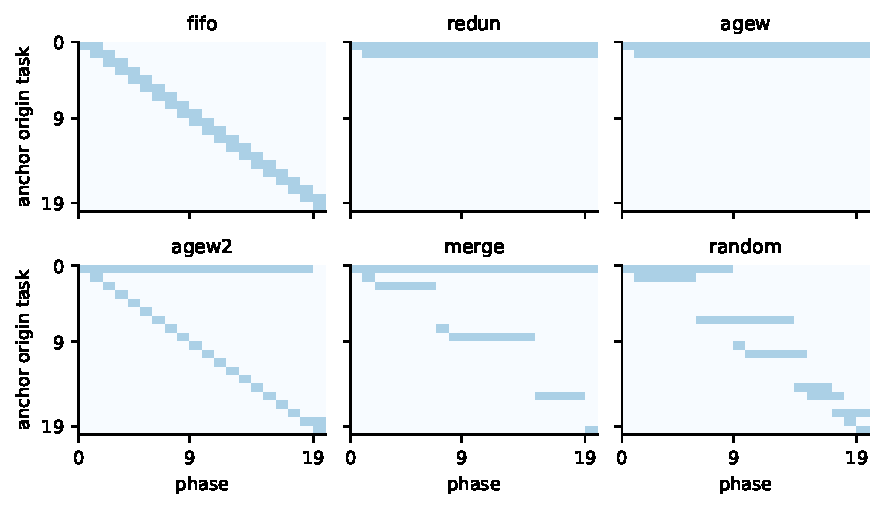
\includegraphics[width=\linewidth]{fig5_cifar_stacktrace.pdf}
\caption{Anchor-stack composition on Split-CIFAR-100 ($T{=}20$,
$M{=}2$, seed 0; all seeds agree on the final sets). Same rendering as
Fig.~\ref{fig:stack}. fifo is a sliding window; redun and agew freeze
on the first anchors (grandfathering); agew2 pairs the oldest with the
newest; merge partially grandfather-protects; random walks down.}
\label{fig:stackcifar}
\end{figure*}

\paragraph{A boundary condition on the mass-keyed failure.}
Unlike on MNIST, the \emph{secondary} effect --- \emph{which}
criterion evicts --- is weak here: fifo $-$ redun is $+1.6$
($t(9){=}2.0$) at $T{=}20$, $M{=}2$, and agew2 $-$ redun is slightly
negative. The reason is structural: under masked-CE training,
forgetting propagates only through the shared trunk, whose low layers
are described similarly by every task's Fisher diagonal; even the
stale anchors $\{\mathcal{A}_1, \mathcal{A}_2\}$ constrain features
later tasks still use, so grandfathering them costs little.
Mass-keyed eviction fails when anchors describe task-specific
structure that goes stale; the primary effect of bounding (recovering
plasticity) survives, while the relative cost of grandfathering
scales with how much low-level structure tasks share --- a testable
prediction for domain-incremental sequences, where the gap should
re-open.

% ============================================================
\section{Discussion}
% ============================================================
\label{sec:discussion}

\paragraph{Why bounding works.}
Eq.~\ref{eq:decomp} says total retention is learning plus transfer.
Unbounded stacks tax learning with stale constraints. A FIFO window
keeps only the freshest $M$ constraints, whose $\theta^{(k)}$ are
near $\theta^{\text{now}}$ and whose Fisher mass is relevant to the
current basin: the penalty constrains what actually needs
constraining.

\paragraph{The mass signal is not useless --- it is mis-keyed.}
redun asks ``which anchor constrains least \emph{now}?''; the honest
answer at eviction time is ``the one just created'', which is exactly
the wrong anchor to drop. agew2 shows mass adds marginal, unstable
value as a secondary signal. The information structure of the
problem makes age the only reliable primary key: eviction-time mass
confounds relevance with staleness.

\paragraph{Protection state as a knowledge base.}
The perspective that unifies these findings is to treat the anchor
stack as a knowledge base rather than an accumulator. A knowledge base
is expected to state \emph{what} it knows, \emph{since when}, and to
support explicit maintenance operations --- eviction, merge, audit ---
over named entries. An unbounded anchor stack violates all three
expectations: it grows without bound, weights all entries equally
regardless of age, and offers no interface for inspection. The
bounded-stack family restores them: each anchor carries an origin tag,
the survivor history records every maintenance event, the eviction
policy is an explicit, swappable choice, and the log-linear law of
Sec.~\ref{sec:exp-law} prices the knowledge retained per horizon
unit. In this reading, the anchor accumulation problem is not an
implementation bug in \delp{}; it is what happens to \emph{any}
protection scheme whose knowledge base lacks a curation policy ---
and the same reading explains why the discounted posterior of online
EWC, which answers the same curation question with an implicit decay,
is interchangeable with the explicit window in accuracy but inferior
in auditability.

\paragraph{Limitations.}
(1) Task-incremental sequences (permuted MNIST, Fashion-MNIST,
Split-CIFAR-100 with a masked head); domain-incremental settings,
where tasks share nearly all low-level structure, may shrink the
age-over-mass gap further (Sec.~\ref{sec:exp-cifar}). (2) $T \le 20$;
the $\ell$-recovery trend grows with $T$ but the BWT cost does too.
(3) All MNIST arms share an uncalibrated hidden gain, as in the audit;
the CIFAR study uses its own protocol with $\lambda$ calibrated on
unbounded \delp{} only; conclusions are within-family comparisons.
(4) Merge's penalty change is measured by instrumentation
(Sec.~\ref{sec:exp-merge}), not bounded formally; a closed-form error
bound is future work. (5) On Split-CIFAR-100 the no-protection reference
outperforms every protection arm
(Sec.~\ref{sec:exp-cifar}): task-incremental evaluation makes
forgetting cheap, so the anchor pathway is a net tax there and the
budget result is internal to protected arms.
(6) The three benchmarks are the standard continual-learning
benchmarks of the regularizer literature, not large-scale vision
models: we do not evaluate ImageNet-scale class-incremental streams, so
the magnitude of the anchor-accumulation cost in that regime is
unmeasured. We regard the diagnosis, not the repair, as the transferable
claim here --- the accumulation law of Sec.~\ref{sec:exp-law}
follows from the regularizer's form rather than from the task
distribution, and should therefore scale; establishing the
corresponding magnitudes at scale is the next step, and the
instrumentation used here (anchor-stack survivor histories, per-run
penalty traces) is designed to be portable to that setting.

% ============================================================
\section{Conclusion}
% ============================================================
\label{sec:conclusion}

Bounding the anchor stack converts the diagnosed anchor accumulation
problem into a control knob: FIFO eviction recovers the learning
term at a declared BWT cost, the budget's effect is structurally
different from $\lambda$'s, age is the only sound eviction signal,
and merge decouples memory from behavior. The effects replicate
across three benchmarks --- permuted and class-incremental, MLP- and
ResNet-based --- with the age-over-mass advantage bounded by a stated
boundary condition on task relatedness, and the protection pathway
itself bounded by a no-protection reference on Split-CIFAR-100.
Single-anchor schemes cannot accumulate the problem by construction,
and a discounted posterior --- itself a soft bound, its mass
converging to a horizon of ${\approx}\,1/(1-\gamma)$ tasks --- recovers
plasticity through the same law: across soft and hard bounds the
learning term falls log-linearly with the protected-mass horizon at
the calibrated $\lambda$ (monotone at every grid value), and a tuned
discount overtakes the window on accuracy at matched forgetting.
Bounding accumulated anchor mass, not the eviction mechanism, is the
active ingredient; the explicit window is the variant whose protection
set is auditable and whose policy is a choice.
Protection schemes for
continual learning should ship with bounded --- or at least
mergeable --- anchor state whenever protection is warranted at all;
the Split-CIFAR-100 reference (Sec.~\ref{sec:exp-cifar}) shows that
the warrant itself is regime-dependent and must be checked first.

% Appendices A (statistics rationale + hyperparameters) and B (full
% per-task accuracy matrices) have been moved to supplementary.tex,
% compiled and submitted as a separate supplementary PDF.

\section*{CRediT authorship contribution statement}
\textbf{Ranxi Zhou:} Conceptualization, Methodology, Software,
Investigation, Formal analysis, Data curation, Writing --- original
draft, Writing --- review \& editing, Visualization.

\section*{Declaration of competing interest}
The author declares that he has no known competing financial interests
or personal relationships that could have appeared to influence the
work reported in this paper.

\section*{Funding}
This research did not receive any specific grant from funding agencies
in the public, commercial, or not-for-profit sectors.

\begin{sloppypar}
\section*{Data availability}
All code, experiment scripts, and the complete JSON records of every
run (including per-phase accuracy matrices and anchor-stack survivor
histories) are publicly available at
\url{https://github.com/zhouranxi/delp-anchor-budget}. This manuscript
and its full reproducibility package --- including the audit scripts
that re-derive every quoted number from those records --- are archived
on Zenodo (doi:10.5281/zenodo.23668522). The precursor audit study is
archived at doi:10.5281/zenodo.23572226 and the companion
segment-specialization audit at doi:10.5281/zenodo.23637972; the
underlying dataset and code release is
doi:10.5281/zenodo.23639561.
\end{sloppypar}

\section*{Declaration of generative AI and AI-assisted
technologies in the manuscript preparation process}
During the preparation of this work, the author used AI-assisted
language-editing tools in order to improve the grammar, clarity, and
consistency of the manuscript text. After using these tools, the
author reviewed and edited the content as needed and takes full
responsibility for the content of the published article. The use of
AI tools did not extend to any scientific content: all experimental
design, analysis, figures, and results were produced and verified by
the author.

\bibliographystyle{elsarticle-num}
\bibliography{refs}

\end{document}
